\subsection{Solver loop}

Here we describe the implementations provided for each step of the algorithm. Most of the details are explained in a side document~\citep{cati}. We only give a quick overview here.

\subsubsection{\texttt{RateContainer} classes}

\begin{figure}[!h]
  \centering
  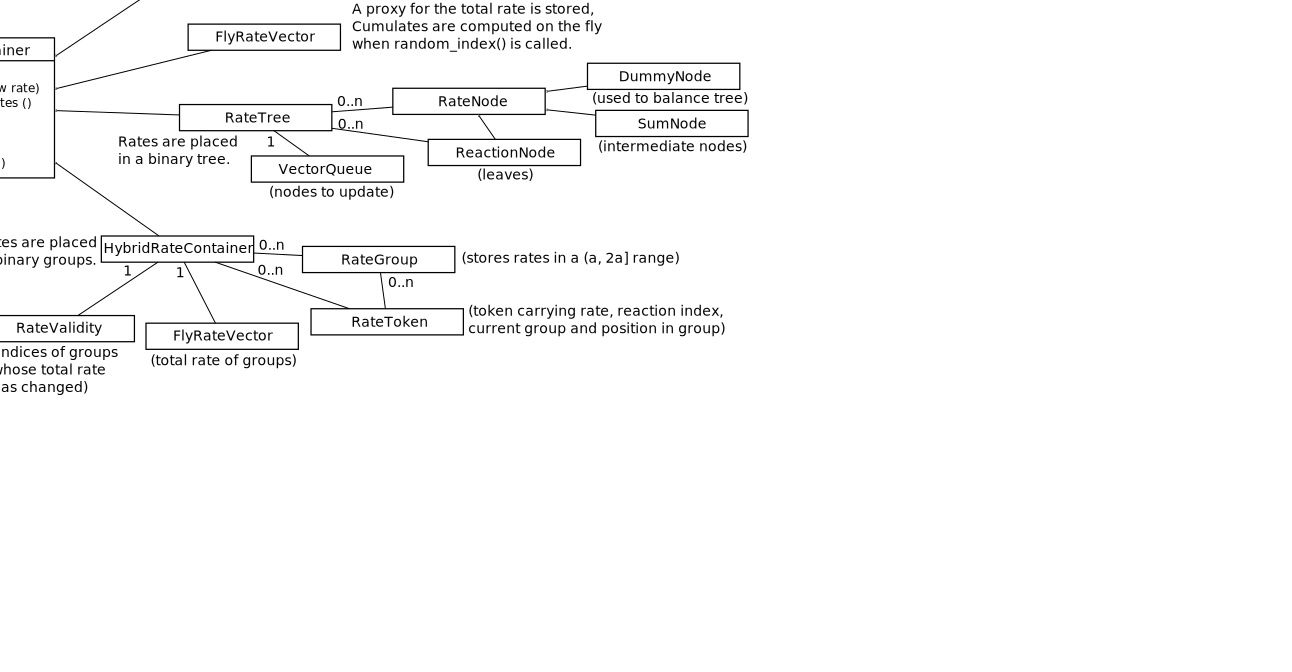
\includegraphics[width=\linewidth]{rate_container}
  \caption{Implementations provided to store rates and perform a multinomial drawing. Implicitly, all theses classes use \texttt{RandomHandler} to perform their random drawings. }
  \label{fig:rate_container}
\end{figure}

We start with the lowest level classes, which perform one of the central tasks of the Gillespie algorithm: drawing a reaction from reaction rates. For efficiency reasons, we propopose several implementation of the algorithm~\reffigp{fig:rate_container}. Comparison and description of theses classes are given in~\citet{cati}. 

Note that multinomial drawing occurs within the solver loop, but also within some reactions such as \texttt{Loading} or \texttt{SequenceBinding}, so these classes are used quite extensively throughout the simulation.

\paragraph{Perspectives} These classes are the most sensitive classes from a numerical point of view. Stability of implementation should be checked more thouroughly (postconditions and or unit tests). \texttt{HybridRateContainer} needs a parameter to work. It is user provided for the moment but I think it should be determined automatically, probably by extending the group structure dynamically.

\subsubsection{\texttt{RateManager} classes}

\begin{figure}[!h]
  \centering
  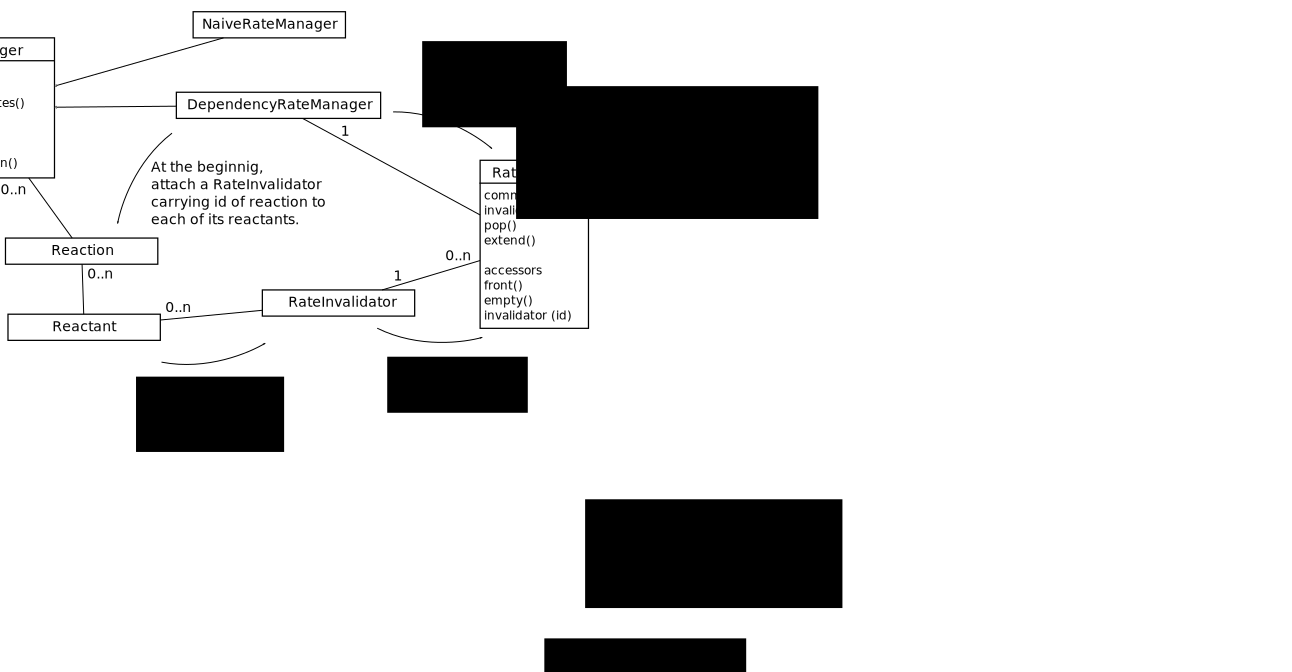
\includegraphics[width=\linewidth]{rate_manager}
  \caption{Implementations provided to update reaction rates. Note that the drawing part of the algorithm is always delegated to a \texttt{RateContainer}. \texttt{DependencyRateManager} uses an Observer pattern to monitor which rates have changed.}
  \label{fig:rate_manager}
\end{figure}

The second layer of the solver loop ensures that the rates are updated when needed to. Two implementations are proposed for this task~\reffigp{fig:rate_manager}. The \texttt{NaiveRateManager} updates every rate. While it is inefficient, it can be used as a reference to test other managers.

\paragraph{Perspectives} While \texttt{DependencyRateManager} performs fairly well in the general case. It is particularily inefficient if there is a molecule $A$ involved in a lot of reactions because a lot of rates have to be recomputed. It could be interesting to pool the reactions involving $A$ into a \texttt{RateContainer} of their own, the latter containing only the contribution to the rate of the \emph{other} reactants. The total rate of reactions involving $A$ would then be the total rate of the container multiplied by the concentration of $A$. This would be viewed by the system as \emph{one} mega reaction. When the concentration of $A$ changes, virtually \emph{nothing} is recomputed, except the total rate of the mega reaction (we suppose the contribution of other reactants has remained constant). If the mega reaction is to be performed, the \texttt{RateContainer} is used to draw which reaction will actually be performed according to their contributions. This change is not possible with the current architecture, the definition of \texttt{RateManager} and the computation of rates would have to be changed.

\subsubsection{\texttt{Solver} classes}

\begin{figure}[!h]
  \centering
  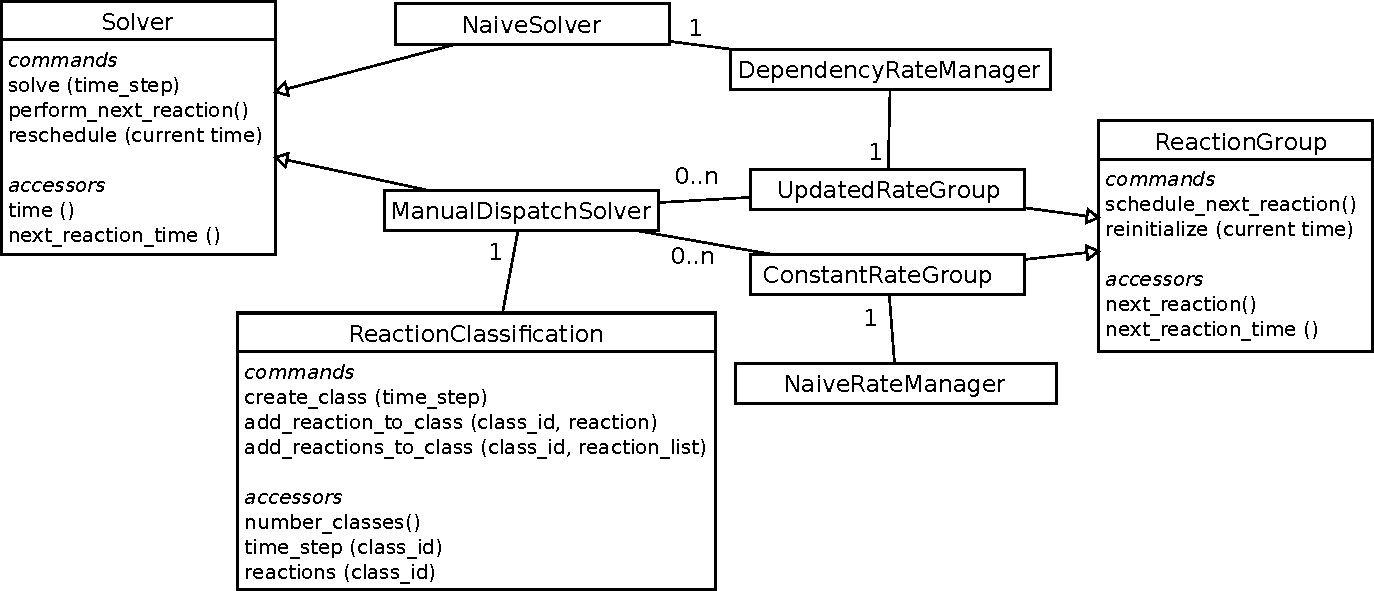
\includegraphics[width=\linewidth]{solver}
  \caption{Two implementations of the \texttt{Solver} class organizing rate updating. \texttt{NaiveSolver} forces recomputation of rates at each time step. \texttt{ManualDispatchSolver} puts reactions into groups: reactions in \texttt{UpdatedRateGroup} are updated after every reaction while those in \texttt{ConstantRateGroup} only at user-defined steps defined in \texttt{ReactionClassification}. Note that all \texttt{Solver} classes use at leaste a variant of \texttt{RateManager} at some point to delegate storing and updating of rates.}
  \label{fig:solver_details}
\end{figure}

For the moment, only one solver class is fully available to the user, \texttt{NaiveSolver}, which implements the exact Gillespie algorithm. Another variant called \texttt{ManualDispatchSolver} is implemented, were the user can assign a time step to each reaction at which its rate will be updated~\reffigp{fig:solver_details}. However, when the rate of a reaction is a constant, there is a risk that its reactants will run out and the reaction will be impossible to realize or reactant number will become negative. In the simulator, the latter case is forbidden, so \texttt{ManualDispatchSolver} ignores reactions impossible to perform due to reactant inavailability. 

\paragraph{Perspectives} There is no user interface to \texttt{ManualDispatchSolver} so it is not really possible to use it in practice witout changing the program. It would probably be more interesting to implement a variant or several variants of \textbf{tau-leaping}, which automatically assigns time steps to reaction to avoid reactant shortage. This has to be done carefully, the variant chosen must be effective event if the number of a chemical becomes or remains fairly low.

